\begin{frame}
\frametitle{The \textit{Discrete View} of A Function} 
\framesubtitle{The $\leq 1$-Arrow Out Property}
\label{slide:discrete-function-view-1}
\begin{itemize}
\item One View: A \alert{Binary Relation} with The \alert{``$\leq1$ Arrow Out''} Property Between Elements of Sets, Say, $A,B$ (on The \textit{Relation Diagram}).
\visible<2-> 
{
\begin{figure}[H]
\centering
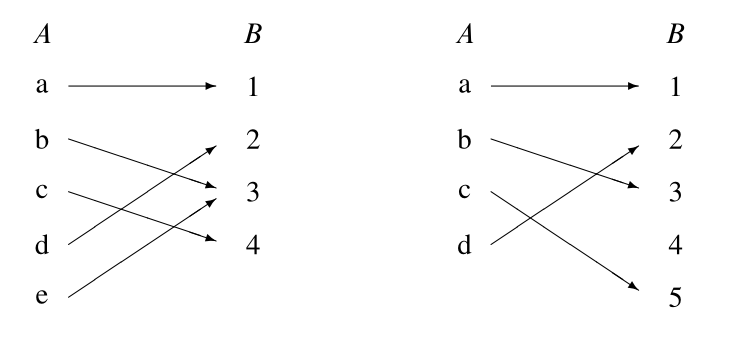
\includegraphics[width=.6\textwidth]{images/function-ex}
\caption{Examples of Function}
\label{fig:functionex}
\end{figure}
}
\item<3-> This Is \alert{Discrete (Table) View of A Function}: Each Discrete Point of \alert{Domain ($A$)} Corresponds to A Discrete Point of \alert{Codomain\footnote{Some Call It `Range'.} ($B$)}:$(a,1),(b,3),(e,3),\dots$.
\end{itemize}
\end{frame}
